%% ===========================================================================
\section{Problem formulation and method}
\label{sec:method}
%% ===========================================================================

\subsection{Proposer--judge formulation}
\label{sec:formulation}

\begin{figure}[pos=t]
\centering
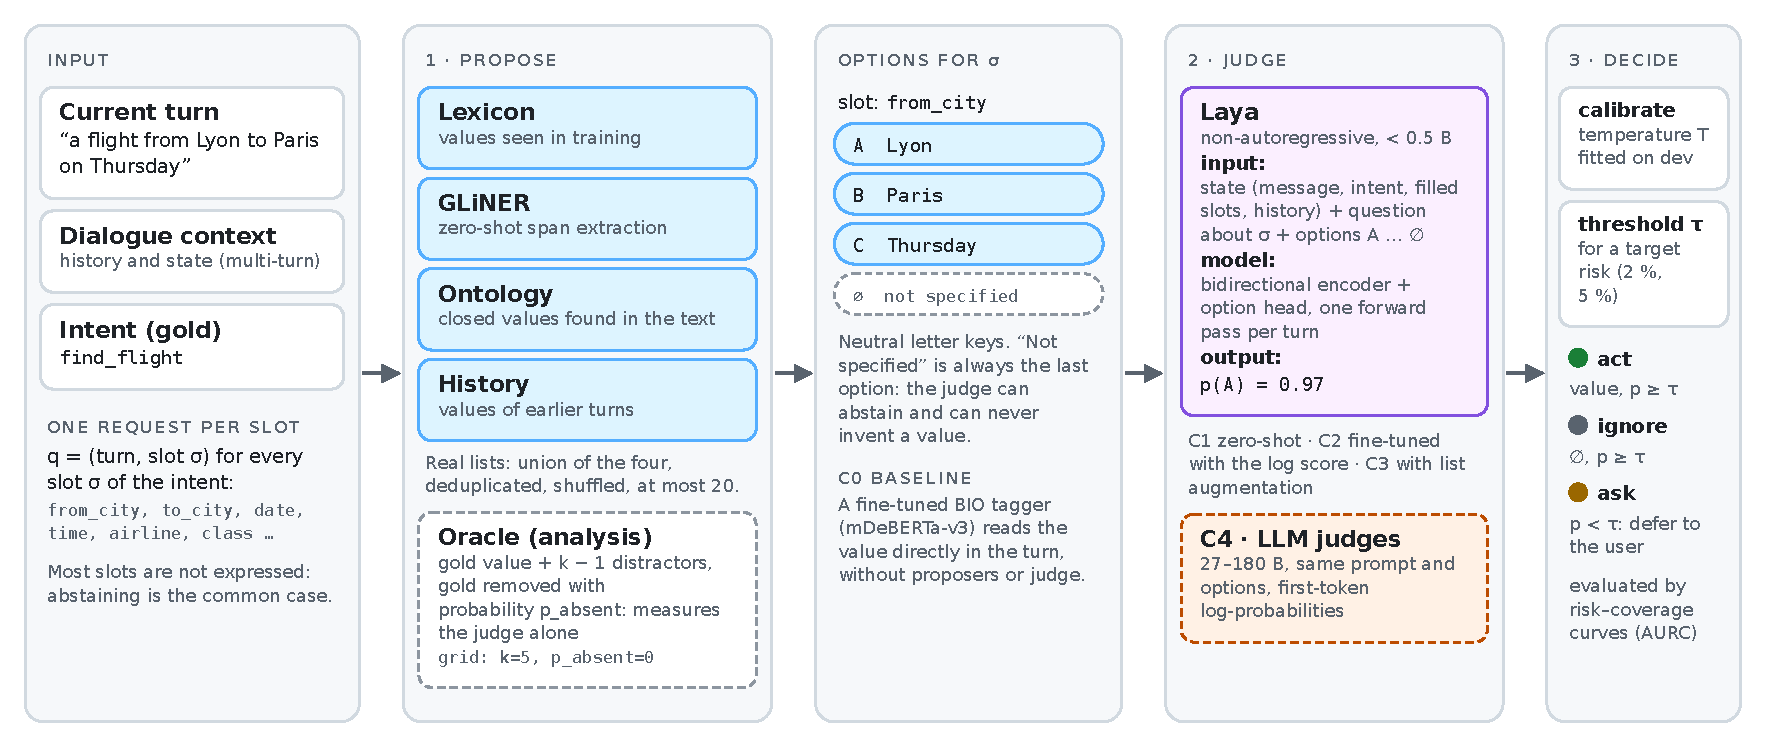
\includegraphics[width=\textwidth]{figures/architecture.pdf}
\caption{The proposer--judge architecture, illustrated on one request: the slot \texttt{from\_city} of the turn ``a flight from Lyon to Paris on Thursday''. \textbf{Input}: one request is issued for every slot of the gold intent, and most of these slots are not expressed. \textbf{1~Propose}: four inexpensive proposers (lexicon of training values, GLiNER, ontology, dialogue history) build the real candidate list; for analysis, an oracle builds a list around the gold value with $k-1$ distractors and removes the gold value with probability $p_{\text{absent}}$. \textbf{Options}: candidates appear under neutral letter keys, followed by ``not specified'' (\none); the distractor C (\emph{Thursday}) is the value of another slot of the same turn, the typical trap of real lists. \textbf{2~Judge}: Laya reads the dialogue state, the question about the slot and the options, and returns a probability per option in one forward pass (C1 zero-shot, C2 fine-tuned, C3 fine-tuned with option-list augmentation); in C4, an LLM judge is scored on the same options. \textbf{3~Decide}: after temperature scaling fitted on development data, a threshold $\tau$ set for a target risk maps the answer to \emph{act} (fill the slot), \emph{ignore} (leave it empty) or \emph{ask} (defer to the user). C0, a fine-tuned BIO tagger, is the classical alternative that reads values directly in the turn, without proposers or judge.}
\label{fig:architecture}
\end{figure}

An \emph{example} $x$ is a user turn: the current utterance $u$, the preceding dialogue history $h$ (empty for single-turn datasets), the current intent or domain $\iota$, and, in multi-turn dialogue, the slots already filled before the turn, $s^{-}$. The schema gives, for each intent $\iota$, the set $\mathcal{S}(\iota)$ of slots that it allows; each slot $\sigma$ has a name and a short natural-language description (\cref{app:conversion}). The gold annotation assigns to each slot either a set of values $V^{*}(x,\sigma)$ expressed in the turn, or nothing.

\Cref{fig:architecture} gives an overview of the architecture on a concrete request; this section formalises it. For every slot $\sigma \in \mathcal{S}(\iota)$ we issue one \emph{request} $q=(x,\sigma)$. A set of proposers $G_1,\dots,G_m$ produces a candidate list
\begin{equation}
  \Cand(q) = \operatorname{dedup}\bigl(G_1(q) \cup \dots \cup G_m(q)\bigr) = (c_1,\dots,c_k), \qquad k \le K,
\end{equation}
where values are normalised before deduplication (\cref{app:conversion}) and the first generator wins ties. A judge $J$ maps the request and its list to a probability distribution over the $k$ candidates and an extra option $\none$ (``not specified''):
\begin{equation}
  p(\cdot \mid q) = J\bigl(x,\sigma,\Cand(q)\bigr) \in \Delta^{k}, \qquad
  \hat{y}(q) = \arg\max_{y \in \Cand(q)\cup\{\none\}} p(y \mid q), \qquad
  \hat{c}(q) = \max_{y} p(y \mid q).
\end{equation}
The predicted value is $\hat{y}(q)$ unless $\hat{y}(q)=\none$, in which case the slot stays empty. An empty list yields $\none$ without calling the judge. The correct option is
\begin{equation}
  y^{*}(q) =
  \begin{cases}
    c_i & \text{if } V^{*}(x,\sigma) \neq \emptyset \text{ and } c_i \in V^{*}(x,\sigma),\\
    \none & \text{otherwise (slot not expressed, or gold value absent from the list).}
  \end{cases}
\end{equation}
Two properties follow directly. The judge cannot output a value that was not proposed, so it cannot hallucinate. And every error falls into exactly one of three classes, which we measure separately (\cref{fig:decomposition,sec:metrics}): a \emph{recall} error (the gold value is not in $\Cand(q)$), a \emph{choice} error (it is in the list but another option is chosen, possibly $\none$), or a \emph{false positive} (a value is chosen for a slot the user did not express).

\begin{figure}[pos=t]
\centering
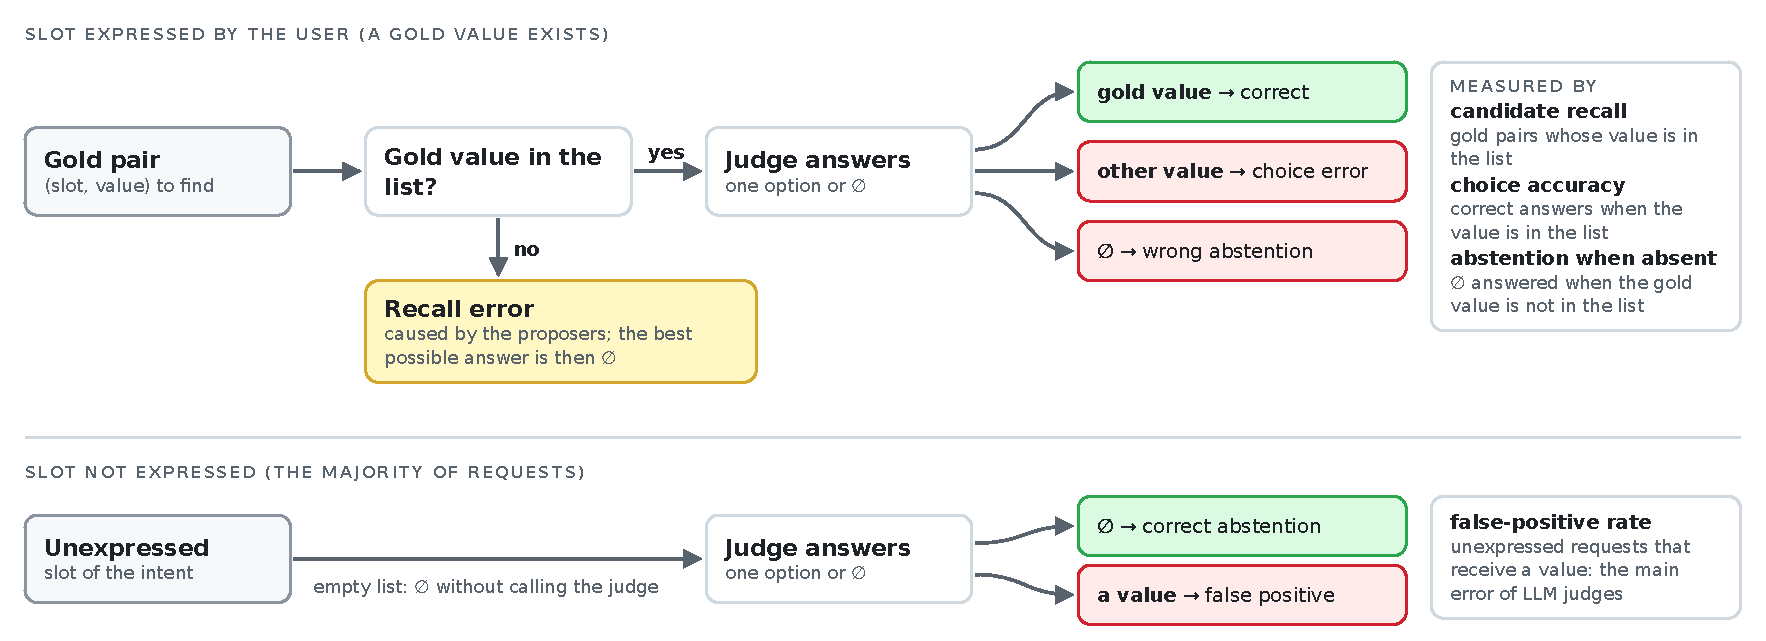
\includegraphics[width=\textwidth]{figures/decomposition.pdf}
\caption{Error decomposition: each request ends in exactly one outcome. \textbf{Top}, a slot expressed by the user: either the gold value is missing from the list, a \emph{recall} error of the proposers for which abstaining is the best possible answer, or it is present and the judge chooses it (correct), chooses another value (\emph{choice} error) or abstains wrongly. \textbf{Bottom}, an unexpressed slot, the majority of requests: the judge must answer \none, and any value is a \emph{false positive}; an empty list is answered \none\ without calling the judge. The measures on the right separate the proposers (candidate recall) from the judge (choice accuracy, abstention when the gold value is absent, false-positive rate).}
\label{fig:decomposition}
\end{figure}

\subsection{The Laya judge}
\label{sec:laya}

Laya \citep{laya2026} is a non-autoregressive decision model released under the Apache-2.0 licence. It encodes a structured \emph{state} (a dictionary of text fields) together with one or more \emph{questions}; each question has typed options rendered as ``\texttt{key: description}'', and a head attached to marker tokens returns a probability distribution over the options of each question in a single forward pass. We use the \texttt{multilingual} checkpoint, built on mmBERT-base \citep{marone2026mmbert} (the English checkpoint is built on ModernBERT-large \citep{warner2025modernbert}), with the runtime pinned to version 0.3.22 and the checkpoint to revision \texttt{7b928d8}. Its encoder accounts for 322\,M parameters for the multilingual checkpoint (mmBERT-base; 421\,M for the English one, according to the model cards), hence ``fewer than half a billion'' parameters in total.

\paragraph{State} The state sent to Laya contains, in this order (Laya truncates a state from the right): the last user message (at most 1,000 characters), the current intent (or domain), the slots already filled (multi-turn only) and the last four turns of history (at most 1,500 characters, truncated from the left).

\paragraph{Question} In the main \emph{single} mode, each request becomes one multiple-choice question whose instruction reads
\begin{quote}\small
\texttt{Which value does the user's last message give for the slot "\{slot\}" (\{description\})?}
\end{quote}
with the candidates as options under neutral letter keys (A, B, \ldots) and a last option ``\texttt{not specified: the last message gives no value for this slot}''. Candidates are shuffled with a seed that depends only on the run seed, the example and the slot, because Laya, like LLM judges \citep{wang2024fair}, has a strong position bias. At most 15 candidates are shown during training and up to 20 during evaluation (\cref{app:hyper}). A \emph{two-step} mode, which first asks whether the slot is expressed and then which candidate is correct, is implemented (\cref{app:prompts}), but its fine-tuned version was not evaluated in this study (hypothesis H4 remains open). All questions of the requests that share a state (same example, intent and filled slots) are grouped into one forward pass: one Laya call per turn.

\subsection{Candidate generation}
\label{sec:candidates}

\paragraph{Oracle candidates} To measure the judge alone, the oracle generator returns the gold value plus $k-1$ distractors, and removes the gold value with probability $p_{\text{absent}}$ when the slot is expressed. Distractors are drawn by a sampler that mixes several strategies, each with a weight: values of the same slot seen in training (\texttt{train\_values}), closed values of the ontology, values of \emph{other} slots of the same utterance (\texttt{other\_slots}), content $n$-grams of the utterance ($n\le 3$), and values from the dialogue state or history. Within a strategy, a value is drawn with probability proportional to $\exp(\mathrm{sim}/0.1)$, where $\mathrm{sim}$ is the character-trigram similarity with the gold value, which yields \emph{hard} distractors. Our main preset, \texttt{hard\_no\_overlap}, additionally excludes boundary variants, i.e.\ values that contain the gold value or are contained in it as whole words (``on april'' or ``april 1'' for ``april''): choosing such a variant is a segmentation error rather than an understanding error, and with real candidates such variants appear naturally when a generator segments badly. The \texttt{hard} preset keeps them and serves as an ablation; the \texttt{easy} preset draws uniformly among all known values of all slots; the \texttt{confusion} preset (used for augmentation, \cref{sec:augmentation}) puts a weight of 3 on \texttt{other\_slots}. Candidates are ``blind'' (no score, source or offsets), so that a judge cannot recognise the gold value from metadata. Three independent random streams, all derived from (seed, example, slot), decide the removal of the gold value, the sequence of distractors and the final order. Lists for $k$ are therefore prefixes of lists for $k+1$, and examples without gold value are nested when $p_{\text{absent}}$ grows, so that sweeps over $k$ and $p_{\text{absent}}$ compare paired conditions.

\paragraph{Real candidates} To measure the whole pipeline, we use the union of four generators, in this priority order: (i) a \emph{lexicon} of the normalised values seen in training for the slot, matched against the $n$-grams of the utterance; (ii) GLiNER \citep{zaratiana2024gliner} (\texttt{urchade/gliner\_multi-v2.1}), zero-shot, with the slot description as label and a threshold of 0.3; (iii) the \emph{ontology}, whose closed values are matched exactly or approximately (similarity $\ge 0.85$) in the utterance; and (iv) the \emph{history} (Multi3WOZ only): the value already in the state, the same attribute in another domain, and known values mentioned in recent turns. The union keeps at most $K=20$ candidates, deduplicated by normalised value, in a shuffled order. The fine-tuned judges are \emph{not} retrained on real candidates: real lists are an out-of-distribution test of the judge trained on oracle lists.

\subsection{Fine-tuning by the log score}
\label{sec:finetuning}

\paragraph{Objective} The released Laya package does not include its training module; the original model was trained with policy-gradient rewards derived from strictly proper scoring rules \citep{laya2026}. We fine-tune it with direct supervision instead: the loss of a question with options $o_1,\dots,o_n$ and correct option $o_{t}$ is the log score $-\log p(o_{t})$ \citep{gneiting2007scoring}, i.e.\ the cross-entropy over its options. This is the same family of strictly proper rules, optimised by supervised learning rather than by reinforcement. We reimplemented the training loop on top of Laya's inference primitives (state encoding, collation and decision head), so that the encoding of a question at training time is exactly the one used for prediction, and we save checkpoints in Laya's own format.

\paragraph{Items built by the inference code} Every training request goes through the function that prepares Laya's questions at evaluation time: same state, same instruction templates, same shuffled order, same truncation of the candidate list. Only the target is added: the position of the gold value among the options, or the ``not specified'' option when the slot is not expressed or the gold value is not in the list. A format mismatch between training and evaluation is therefore impossible by construction. Training requests are built on the training split with the evaluation's request builder (all slots allowed by the gold intent, \cref{sec:setup}).

\paragraph{Class imbalance} Most requests concern slots that the user did not express (about 94\% on MultiATIS++). We keep all requests with an expressed slot and at most two unexpressed requests per expressed request in each example (\texttt{unexpressed\_ratio} $=2$), drawn with the run seed; this gives 43,000 to 189,000 training questions per dataset and language (\cref{tab:trainsizes}). On MultiATIS++ English this yields 43,007 training questions from 4,478 training utterances.

\paragraph{Optimisation and checkpoint selection} We train for three epochs with AdamW (learning rates $2\times10^{-5}$ for the encoder and $10^{-4}$ for the head), a linear warm-up over 5\% of the steps followed by cosine decay, batches of 32 questions, gradient clipping at 1.0, bf16 autocast over fp32 weights and gradient checkpointing (\cref{tab:hyper}). After each epoch we evaluate the slot F1 on all requests of the first 300 development examples (same distribution as at test time) and keep the best epoch. We first selected on the development loss, but the loss is distorted by over-confidence: one C3 seed kept an epoch whose loss was lower but whose decisions were worse; selecting on development F1 removed this failure mode (\cref{sec:threats}). Checkpoints are saved with neutral temperatures ($T=1$); calibration is a separate, post-hoc step (\cref{sec:decision}).

\paragraph{Bilingual training} For the joint English--French condition, the items of both languages are concatenated; each language keeps its own ontology (slot descriptions in that language where available) and its own oracle candidates fitted on its own training split. The checkpoint is selected on the English development set, with oracle candidates. The main configuration uses \emph{monolingual} models (one per dataset and language); bilingual training and English-to-French transfer are analysed in \cref{sec:rq3}, where bilingual training turns out to be unstable with real candidates.

\subsection{Option-list augmentation}
\label{sec:augmentation}

A judge trained on a single list shape (oracle, $k=5$, gold always present) may fail when the context changes: longer lists, a missing gold value, other kinds of distractors. Our augmentation draws, for each training example, one combination of list size, missing-value rate and distractor preset, uniformly among the Cartesian product of the following lists (the order of options is already shuffled by the judge):
\begin{itemize}
  \item \textbf{C3 v1} (generic): $k\in\{2,5,10,20\}$, $p_{\text{absent}}\in\{0, 0.2, 0.5\}$, distractors $\in\{\texttt{easy},\texttt{hard\_no\_overlap}\}$;
  \item \textbf{C3 v2} (confusion-oriented): $k\in\{2,2,3,3,5,10,20\}$ (short lists twice as likely), $p_{\text{absent}}\in\{0, 0.2, 0.5\}$, distractors $\in\{\texttt{confusion},\texttt{hard\_no\_overlap}\}$.
\end{itemize}
Version~2 was designed after analysing the failure of version~1 on real candidates (\cref{sec:rq5}): real lists are short and their main trap is a value of \emph{another slot} of the same utterance (``boston'' proposed as the stop-over city when it is the departure city), whereas the \texttt{easy} distractors of version~1 are of other types and easy to reject. On 200 training examples, 63\% of the distractors for unexpressed slots come from other slots of the utterance with \texttt{confusion}, against 33\% with \texttt{hard\_no\_overlap}. In the remainder of the paper ``C3'' denotes version~2; version~1 is kept as an ablation of the augmentation design. Note that with the judge's default of 15 options at training time, $k=20$ is truncated to 15 (\cref{app:hyper}).

\subsection{Calibrated three-zone decision}
\label{sec:decision}

\paragraph{Calibration} The unit is a judged request: the judge's distribution over its options and the correct option $y^{*}$. Requests with an empty list are excluded, since their decision ($\none$) is certain and identical for all judges. We fit on development data (i) \emph{temperature scaling} \citep{guo2017calibration}, $p_T(y) \propto p(y)^{1/T}$ with $T$ minimising the negative log-likelihood (NLL), which preserves the ranking of options and hence the decision, and (ii) \emph{isotonic regression} \citep{zadrozny2002transforming} of the correctness of the selected option on its confidence. We report NLL, the multi-class Brier score and the expected calibration error (ECE, 15 equal-width bins).

\paragraph{Decision} For a confidence $\hat c$ and a threshold $\tau$, the policy is
\begin{equation}
  \text{decision}(q) =
  \begin{cases}
    \textsc{act} \ (\text{fill } \hat y) & \text{if } \hat c \ge \tau \text{ and } \hat y \neq \none,\\
    \textsc{ignore} \ (\text{leave empty}) & \text{if } \hat c \ge \tau \text{ and } \hat y = \none,\\
    \textsc{ask} \ (\text{defer to the user or a costlier judge}) & \text{if } \hat c < \tau.
  \end{cases}
\end{equation}
\emph{Coverage} is the share of requests decided without asking and \emph{risk} the error rate among them \citep{geifman2017selective}. Sweeping $\tau$ over all observed confidences (ties treated together) gives the risk--coverage curve, whose area (AURC; lower is better) summarises how well the confidences rank the errors. For a target risk (2\% and 5\% in the main grid), the threshold that maximises coverage is chosen on development data and then applied unchanged. As long as the test set is closed, we split the development set into two halves of clusters (dialogues or utterances), fit on one half, evaluate on the other, in both directions, and average (two folds). For the test-set results (\cref{sec:rq4}), calibration and thresholds are fitted on the whole development set and applied once, unchanged, to the test set.

\subsection{LLM judges}
\label{sec:llmjudge}

The LLM judges play exactly the same role. Each request is rendered with a fixed, versioned prompt (\texttt{slot-judge-v1}, reproduced in \cref{app:prompts}) that contains the slot, its description, the intent, the filled slots, the last four turns of history, the last user message with its language, and the candidates under letter keys followed by a ``not specified'' option, in the same shuffled order as for Laya. The model is asked to answer with a single letter. We generate one token at temperature 0 and read the top-20 log-probabilities of that first token; the probabilities of all tokenisations of a letter (``A'', ``\textvisiblespace A''\ldots) are summed and renormalised over the letters offered. If no letter appears in the top-20, the distribution is uniform and the case is logged (this never occurred in our checks, \cref{sec:llms}). Reasoning (``thinking'') is switched off through the chat template, which we verified per model family. This logit-based reading gives the LLM a full probability distribution over the same options as Laya, which is required for a fair calibration comparison.
